
\section{Introduction}

\paragraph{}LArTPC detectors have the capability of producing three-dimensional high-resolution images of charge deposition, providing calorimetric, as well as millimeter-resolution spatial information on particle-interactions occuring in the detector. With this rich, high-quality data comes the complexity of developing reconstruction tools capable of synthesizing the vast amount of information into a hand-ful of reconstructed quantites which aim to describe the physical variables associated with the particle responsible for the signatures observed in the detector. This task is espeically complex in the case of Electro-Magnetic (EM) showers, which, due to the stochastic nature of electron-Bremsstrahlung and pair-production, significant variability in the appearance of each individual shower makes the development of generic reconstruction algorithms particularly challenging. In this note we aim to summarize the state of shower-reconstruction tools developed for LArTPC detectors.
\paragraph{}EM showers are the signature left by electrons, positrons, and photons as they deposit energy in a LArTPC. Electrons and positrons traversing the argon volume will undergo electron-Bremsstrahlung, producing photons which can carry away a significant fraction of the original electron's energy. Meanwhile, photons in argon will pair-produce leading to an $e^+$/$e^-$ pair. These two phenomena combined lead the single original electron/positron or photon to produce a cascade of particles, which we refer to as an EM shower. The goal of what in this note we define as \texttt{shower-reconstruction} is the task of reconstructing, provided input information pertaining to the visible charge-deposition seen in the detector, the physical quantities associated with the particle that produced the EM shower such as the energy, momentum, 3D vertex, and particle species (electron or photon).
\paragraph{}Across the energy-range that current LArTPC neutrino-detectors are exposed to, from tens of MeV to more than one GeV of energy, showers can appear significantly different. Additionally, the stochastic nature of the Bremsstrahlung process and photon pair-production causes significant variability in how showers manifest themselves in the observable data. Because of this, shower-reconstruction algorithms need to be complex enough to deal with a variable input, and different reconstruction tools may be better geared for different shower energies. Fig.~\ref{fig:emshower_sim} shows a comparison of what a low ($\sim$100 MeV) and high ($\sim$2 GeV) shower might look like.
\begin{figure}[H]
\centering
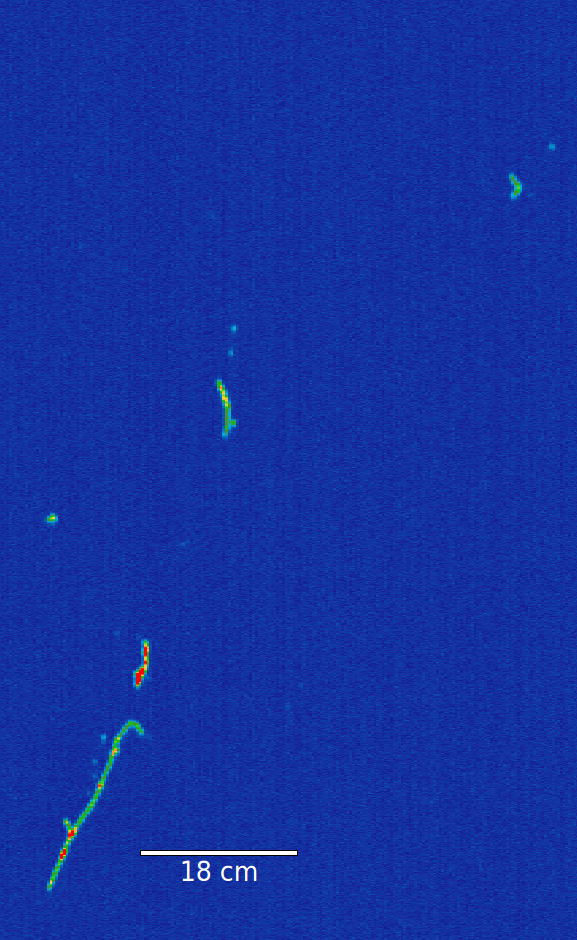
\includegraphics[height=0.45\textwidth]{figures/raw_sim_eminus_139MeV.png}
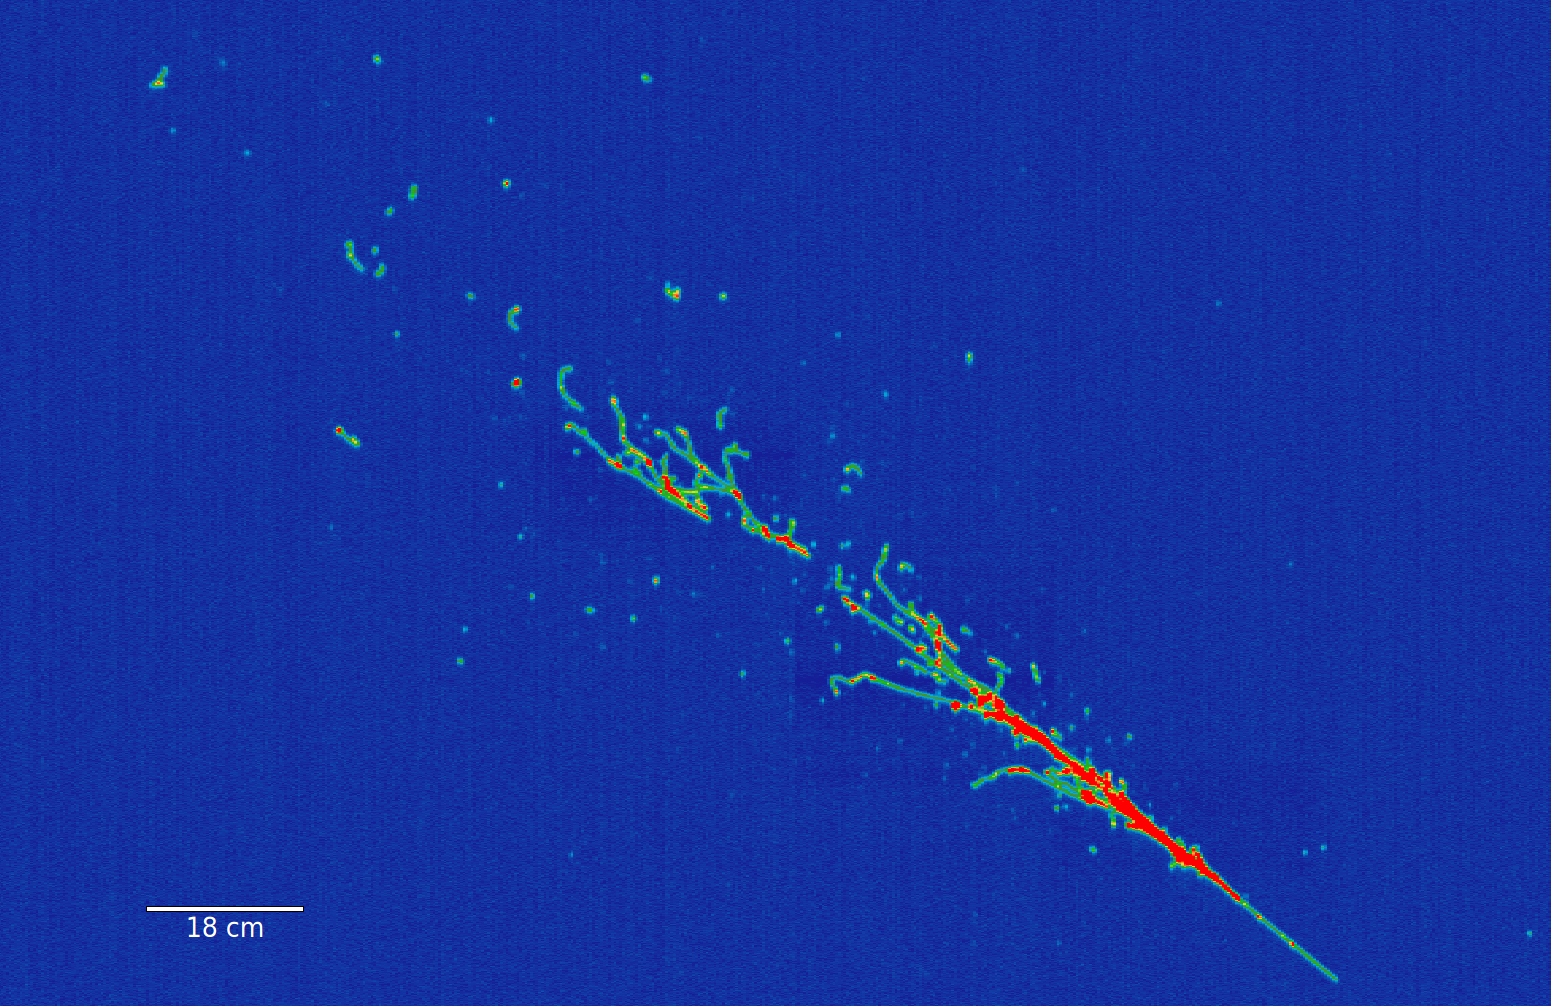
\includegraphics[height=0.45\textwidth]{figures/raw_sim_eminus_1815MeV.png}
\caption{Left: 139 MeV simulated electron EM shower. Right: 1815 MeV simulated electron EM shower.}
\label{fig:emshower_sim}
\end{figure}
\paragraph{}Many reconstruction stages are necessary in order to reconstruct EM showers. Signal processing, hit reconstruction, clustering, and 3D reconstruction are all important steps in this chain. The work of this note only deals with the last element of this chain: the reconstruction of the physical quantities associated with EM showers starting from the 2D and 3D input representing the spatial and calorimetric information associated with the charge deposited by the EM shower. One of the crucial steps in this chain, and arguably the most challenging when it comes to the reconstruction of EM showers, is the clustering of 2D hits, or 3D space-points associated with an EM shower. Current clustering tools are not described in this note, but we reference some of the notes describing this work:~\cite{bib:pandora},~\cite{bib:LArOpenCV}.
\paragraph{}We first aim to provide documentation describing the reconstruction framework developed in order to perform shower reconstruction. This section is perhaps most useful to anyone trying to become familiar with the code in order to start further developing the tools available within the framework. This is done in Sec.~\ref{sec:framework}. We next move on to describing the individual algorithms developed within the framework. This section is meant to be a living document in which, as additional algorithms are written, or old ones developed, their description is updated. This section aims to provide documentation for any analysis using the shower-reconstruction framework, and is probably of interest to anyone wishing to learn how shower-reconstruction is performed for a specific analysis. We point out that the algorithms to be used by a specific analysis may vary, as different algorithms can be combined in different orders. Ultimately it is up to an analysis note to provide a description of what algorithm sequence is used. The description of all algorithms can be found in Sec.~\ref{sec:algos}. We next describe the shower-reconstruction quality tools developed to study the performance of the various reconstruction tools. This section {\color{red} IS CURRENTLY INCOMPLETE} and can be found in Sec.~\ref{sec:quality}.
